% !TeX program = xelatex
% Main talk: title + 12 slides, about 4 min 55 s including clips and Annex B.
% Original template: reference/main-template.tex. Narration: presenter-notes.txt.
\documentclass[aspectratio=169,10pt]{beamer}
\usetheme[nosectionpages]{terminal}
\usepackage{amsmath,amssymb,booktabs,array,tabularx}
\usepackage{appendixnumberbeamer}
\usepackage{pgfplots}
\pgfplotsset{compat=1.18}
\usetikzlibrary{arrows.meta,positioning}
\graphicspath{{./}{images/}}
\setlength{\tabcolsep}{5pt}
\renewcommand{\arraystretch}{1.17}
\newcolumntype{Y}{>{\raggedright\arraybackslash}X}
\newcommand{\evidence}[1]{{\scriptsize\textbf{#1}}\par\smallskip}
\newcommand{\shot}[2]{\includegraphics[width=\linewidth,height=#2,keepaspectratio]{#1}\par}
\newcommand{\key}[1]{\textbf{\texttt{[#1]}}}
\terminalfootprefix{ME5314 / E2}
\terminalwindow{topspin\_investigation.tex}
\terminalshell{\$ replay Top\_spin\\> one recorded trial, four ball locations\\> geometric criterion + proposed judgments}
\title[Recorded-path feasibility]{Can this recorded sweep\\intercept the ball?}
\subtitle{From OpenSim motion analysis to a Vizard affordance investigation}
\author{J. Chambe \quad S. Gonz\'alez \quad L. Kamt}
\institute{UTEC\\ME5314 Sports Engineering \quad Instructor: W. Kim}
\date{November 23, 2026}
\begin{document}
\begin{frame}[plain,noframenumbering]\titlepage\end{frame}
\section{Question and recorded motion}
\begin{frame}{A possibility for this actor and path}
\begin{columns}[T,onlytextwidth]
\begin{column}{0.43\textwidth}
\begin{tbox}{Research question}
Can this recorded racket-proxy sweep intersect a stationary ball as its outward position changes?
\end{tbox}
\par\medskip
\begin{itemize}\small
\item Actor: the captured left-handed player.
\item Environment: table, floor and simulated ball.
\item Scope: feasibility of the recorded path.
\end{itemize}
\end{column}
\begin{column}{0.53\textwidth}
\shot{images/view1.png}{3.85cm}
\par\smallskip
{\footnotesize Recorded skeleton with a hand/forearm proxy. The offset avatar provides a qualitative view.}
\end{column}
\end{columns}
\begin{ibox}A geometric intersection does not establish a successful return.\end{ibox}
\src{Project scene and report; E2 rubric, pp. 1--2}
\end{frame}

\begin{frame}{One trial, two representations}
\begin{columns}[T,onlytextwidth]
\begin{column}{0.53\textwidth}
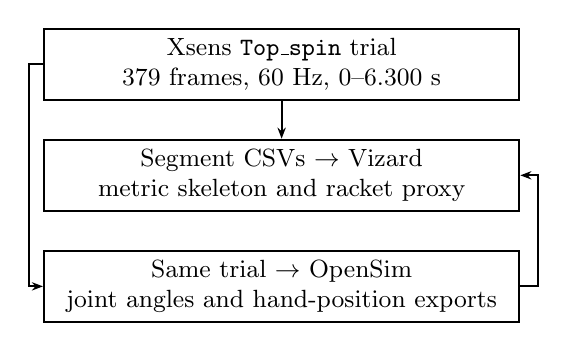
\begin{tikzpicture}[n/.style={draw,thick,fill=white,align=center,text width=5.8cm,minimum height=0.72cm,font=\small},a/.style={-{Stealth[length=4pt]},thick}]
\node[n] (data) {Xsens \texttt{Top\_spin} trial\\379 frames, 60 Hz, 0--6.300 s};
\node[n,below=0.48cm of data] (viz) {Segment CSVs $\rightarrow$ Vizard\\metric skeleton and racket proxy};
\node[n,below=0.48cm of viz] (os) {Same trial $\rightarrow$ OpenSim\\joint angles and hand-position exports};
\draw[a] (data) -- (viz);
\draw[a] (data.west) -- ++(-0.18,0) |- (os.west);
\draw[a] (os.east) -- ++(0.22,0) |- (viz.east);
\end{tikzpicture}
\end{column}
\begin{column}{0.43\textwidth}
\textbf{Scale, axes and timing}
\begin{itemize}\small
\item Position in metres. Angles in degrees.
\item Xsens: forward, left, up.
\item Vizard: right, up, forward.
\end{itemize}
\[(x,y,z)_V=(-y,z,x)_X\]
\begin{itemize}\small
\item Remove initial horizontal pelvis offset. Preserve height.
\item Normal $1.0\times$; labeled slow motion $0.25\times$.
\end{itemize}
\end{column}
\end{columns}
\par\medskip
{\small Vizard reads Xsens CSVs. OpenSim supplies the comparison reference, rather than directly driving the scene.}
\src{Scene data loader and axis mapping; \texttt{Top\_spin-001} OpenSim exports}
\end{frame}

\section{Fidelity}
\begin{frame}{Three frames expose a height mismatch}
\evidence{Recorded screenshots + recomputed export comparison}
\begin{columns}[T,onlytextwidth]
\begin{column}{0.32\textwidth}\centering\textbf{V1: 2.500 s}\par\par\smallskip\shot{V1.png}{2.20cm}\end{column}
\begin{column}{0.32\textwidth}\centering\textbf{V2: 3.083 s}\par\par\smallskip\shot{V2.png}{2.20cm}\end{column}
\begin{column}{0.32\textwidth}\centering\textbf{V3: 3.600 s}\par\par\smallskip\shot{V3.png}{2.20cm}\end{column}
\end{columns}
\par\smallskip\centering\small
\begin{tabular}{@{}lrrr@{}}\toprule
Left hand height (m) & V1 / f150 & V2 / f185 & V3 / f216\\\midrule
OpenSim export & 1.124 & 1.148 & 1.225\\
Vizard skeleton & 1.081 & 1.177 & 1.334\\
Difference (Vizard $-$ OpenSim) & $-0.043$ & $+0.029$ & $\mathbf{+0.109}$\\\bottomrule
\end{tabular}\par
\par\medskip\raggedright\small
The 10.9 cm discrepancy at V3 limits fidelity. Segment/model definitions and alignment need further checking.
\src{Same-row comparison; timestamp offsets $\leq1$ ms. Exact angles and evidence limits in backup A.}
\end{frame}

\section{Controlled investigation}
\begin{frame}{A fixed rule defines interception}
\begin{columns}[c,onlytextwidth]
\begin{column}{0.44\textwidth}
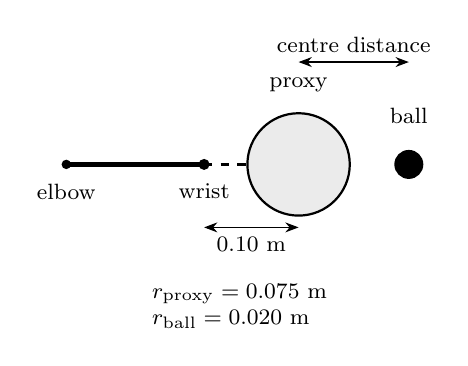
\begin{tikzpicture}[x=1cm,y=1cm,>=Stealth]
\draw[line width=2pt] (-0.2,0)--(1.55,0);
\fill (-0.2,0) circle(0.06);\fill (1.55,0) circle(0.07);
\draw[dashed,thick] (1.55,0)--(2.75,0);
\draw[thick,fill=black!8] (2.75,0) circle(0.65);
\draw[thick,fill=black] (4.15,0) circle(0.17);
\node[below,font=\footnotesize] at (-0.2,-0.12) {elbow};
\node[below,font=\footnotesize] at (1.55,-0.12) {wrist};
\node[above,font=\footnotesize] at (2.75,0.8) {proxy};
\node[above,font=\footnotesize] at (4.15,0.4) {ball};
\draw[<->] (1.55,-0.8)--node[below,font=\footnotesize]{0.10 m}(2.75,-0.8);
\draw[<->] (2.75,1.3)--node[above,font=\footnotesize]{centre distance}(4.15,1.3);
\node[align=left,font=\footnotesize] at (2,-1.8) {$r_{\rm proxy}=0.075$ m\\$r_{\rm ball}=0.020$ m};
\end{tikzpicture}
\par{\scriptsize Schematic, not to scale. No racket sensor was recorded.}
\end{column}
\begin{column}{0.52\textwidth}
\textbf{Independent of observer judgments}
\[D(d)=\min_{i=0,\ldots,378}\left\|\mathbf p_i-\mathbf b(d)\right\|\]
\begin{ibox}Interception if $D(d)\leq0.095$ m\end{ibox}
\small
\[\mathbf b(d)=\mathbf p_{185}+d\,\hat{\mathbf u}_{\rm out}\]
The outward direction runs horizontally from pelvis to proxy at frame 185.
\par\medskip
\begin{itemize}
\item Vary only $d$: 0, 0.08, 0.15, 0.30 m.
\item Fix motion, $1.0\times$ speed, camera and scene.
\item Prediction: C1/C2 intersect; C3/C4 miss.
\end{itemize}
\end{column}
\end{columns}
\src{Scene: \texttt{paddle\_proxy}, \texttt{evaluate}, \texttt{CONDITIONS}}
\end{frame}

\begin{frame}{C2 and C3 straddle the model boundary}
\evidence{Simulated geometry, independently recomputed from 379 recorded frames}
\centering
\begin{tabular}{@{}lrrcrrl@{}}\toprule
 & $d$ (m) & $D$ (m) & Prediction & $t_{\min}$ (s) & Margin (m) & Result\\\midrule
C1 & 0.00 & 0.000 & Possible & 3.083 & $+0.095$ & Intercept\\
C2 & 0.08 & 0.080 & Possible & 3.083 & $+0.015$ & Intercept\\
C3 & 0.15 & 0.150 & No & 3.083 & $-0.055$ & Miss\\
C4 & 0.30 & 0.296 & No & 1.683 & $-0.201$ & Miss\\\bottomrule
\end{tabular}\par
\par\medskip
\begin{columns}[T,onlytextwidth]
\begin{column}{0.49\textwidth}
\begin{tbox}{C2 is close to the threshold}
\small Its positive margin is only 1.5 cm. The 2.9 cm hand-height discrepancy at V2 motivates a sensitivity check, but is not a calibrated proxy-error bound.
\end{tbox}
\end{column}
\begin{column}{0.47\textwidth}
\textbf{The search covers the full trial}\par\par\smallskip
\small C4's nearest approach occurs earlier, at frame 101. It remains a miss. The minimum is not constrained to the reference stroke at frame 185.
\end{column}
\end{columns}
\src{Margin $=0.095-D$; \texttt{evidence/conditions.csv}. Screenshots C1--C4 in backups C--D.}
\end{frame}

\begin{frame}{Playback and all four conditions}
\begin{columns}[c,onlytextwidth]
\begin{column}{0.66\textwidth}
\shot{C1.png}{4.35cm}
\par\par\smallskip{\footnotesize Existing Vizard recording. Metric skeleton, proxy, ball and table.}
\end{column}
\begin{column}{0.30\textwidth}
\small
\key{SPACE} Play / pause\\[6pt]\key{R} Restart\\[6pt]
\key{S} $1.0\times / 0.25\times$\\[6pt]\key{1--4} Conditions\\[6pt]
\key{G} Validation frames\\[6pt]\key{V} Reveal criterion
\par\medskip
\begin{tbox}{Local video links}\footnotesize
\href{run:C1VIDEO.mp4}{Open C1 clip (11.6 s)}\\[6pt]
\href{run:C2,3,4VIDEO.mp4}{Open C2--C4 clip (23.6 s)}
\end{tbox}
\end{column}
\end{columns}
\src{Bundled MP4s; table $2.74\times1.525$ m, height 0.76 m; floor ruler 1 m}
\end{frame}

\section{Ecological interpretation}
\begin{frame}{Viewpoint changes available information}
\begin{columns}[T,onlytextwidth]
\begin{column}{0.49\textwidth}
\centering\textbf{Scene view}\par\par\smallskip\shot{images/view3.png}{2.95cm}
\par\par\smallskip\raggedright\small
Top-down view separates horizontal paths. Vertical separation is harder to judge.
\end{column}
\begin{column}{0.47\textwidth}
\textbf{Candidate optical information}
\begin{itemize}\small
\item Proxy--ball gap and its closure.
\item Trajectory alignment and occlusion.
\item Table edges, floor and ruler as scale references.
\end{itemize}
\par\medskip
\begin{tbox}{One shared environment}
\small Camera position changes projection and visibility. The world-coordinate criterion remains unchanged.
\end{tbox}
\end{column}
\end{columns}
\par\medskip
{\small These are candidate cues. Their use by observers has not been measured.}
\src{Gibson (1979); E2 rubric, p. 2; scene camera definitions}
\end{frame}

\begin{frame}{Possibility, judgment and outcome}
\small
\begin{tabularx}{\textwidth}{@{}p{2.1cm}Yp{3.2cm}@{}}\toprule
Level & Question & Evidence status\\\midrule
Action possibility & Does this modeled recorded sweep geometrically intersect this ball? & Simulated criterion\\[5pt]
Judgment & Does an observer say that interception is possible? & Proposed protocol\\[5pt]
Outcome & Does the struck ball clear the net and land legally? & Not tested\\\bottomrule
\end{tabularx}\par
\par\bigskip
\begin{tbox}{Touch--posture covariation}
In live action, changes in posture covary with contact and inertial forces. That relation supplies haptic information in its own right.
\end{tbox}
\par\smallskip
\textbf{This scene is visual only.} A replay, force label or screw-variable drawing does not demonstrate haptic pickup.
\src{Gibson (1966, 1979); E2 rubric, p. 2}
\end{frame}

\begin{frame}{Judgments remain a proposed experiment}
\evidence{Proposed protocol. No participant responses collected or invented.}
\begin{enumerate}
\item \textbf{Consent and controls.} Three consenting peers, one fixed camera and skeleton view, same trial at $1.0\times$.
\item \textbf{Blind the numerical cues.} Hide criterion, offset labels and console. Randomize four conditions, repeated three times: 12 trials per observer.
\item \textbf{Record before feedback.} \emph{Can this recorded sweep intersect the ball?} Possible / not possible, plus confidence from 1 to 5.
\item \textbf{Compare after all judgments.} Report counts, agreement and false positives/negatives by condition. Treat these as exploratory descriptions.
\end{enumerate}
\par\medskip
\begin{ibox}Geometric classification is available. Perceptual accuracy is unmeasured.\end{ibox}
\src{Proposed implementation of the no-new-participant-data route permitted by the rubric}
\end{frame}

\section{Answer}
\begin{frame}{The replay supports a bounded answer}
\begin{tbox}{Answer to the investigation}
For this recorded trial and spherical racket proxy, ball offsets of 0 and 8 cm intersect the modeled path. Offsets of 15 and 30 cm do not.
\end{tbox}
\par\bigskip
\begin{columns}[T,onlytextwidth]
\begin{column}{0.48\textwidth}
\textbf{What the evidence supports}
\begin{itemize}\small
\item Reproducible recorded-path geometry.
\item A controlled condition comparison.
\item Different optical views of one environment.
\end{itemize}
\end{column}
\begin{column}{0.48\textwidth}
\textbf{Limits on the conclusion}
\begin{itemize}\small
\item Hand-height mismatch reaches 10.9 cm.
\item Racket pose, ball dynamics and adaptation are absent.
\item Judgments and haptic pickup remain untested.
\end{itemize}
\end{column}
\end{columns}
\par\medskip
{\small A stronger test would add direct racket tracking, matched OpenSim pose captures and preregistered observer judgments.}
\src{Finite export check at repository revision \texttt{90abbd9}; no claim of maximum reach}
\end{frame}

\section{Shannon information theory}
\begin{frame}{Annex B: entropy of speed occupancy}
\evidence{Recorded kinematics. Three windows of 31 frames around peak proxy speed.}
\begin{columns}[c,onlytextwidth]
\begin{column}{0.50\textwidth}
\begin{tikzpicture}
\begin{axis}[width=6.7cm,height=4.2cm,xmin=0,xmax=6.3,ymin=0,ymax=9.2,
xlabel={Time (s)},ylabel={Proxy speed (m/s)},grid=major,grid style={black!10},
tick label style={font=\footnotesize},label style={font=\footnotesize}]
\addplot[black,thick] table[x=time_s,y=proxy_speed_m_s,col sep=comma]{evidence/speed-series.csv};
\addplot[only marks,mark=*,mark size=2pt] coordinates {(1.683333,7.716825)(3.083333,7.836990)(4.333333,7.260554)};
\node[font=\scriptsize,anchor=south] at (axis cs:1.683333,7.8) {S1};
\node[font=\scriptsize,anchor=south] at (axis cs:3.083333,7.9) {S2};
\node[font=\scriptsize,anchor=south] at (axis cs:4.333333,7.35) {S3};
\end{axis}
\end{tikzpicture}
\end{column}
\begin{column}{0.46\textwidth}
\[
H=-\sum_{k=1}^{8}p_k\log_2p_k
\]
{\small $p_k$: fraction of window frames in speed bin $k$; bins are 1 m/s wide.}
\par\medskip
\centering\small
\begin{tabular}{@{}lrr@{}}\toprule
 & Bits & Nats\\\midrule
Whole trial & 2.443 & 1.693\\
S1 & 2.877 & 1.994\\
S2 & 2.868 & 1.988\\
S3 & 2.922 & 2.025\\\bottomrule
\end{tabular}\par
\par\par\smallskip
$H_{\rm nats}=H_{\rm bits}\ln2$
\end{column}
\end{columns}
\par\smallskip
\small Maximum: 3 bits for eight equally occupied bins. High entropy means a more spread-out speed distribution, not demonstrated skill or success.
\src{Claude E. Shannon; group report Annex B; recomputed histogram occupancy}
\end{frame}

\begin{frame}{Location reduces outcome uncertainty}
\evidence{Annex B: simulated criterion across 3 stroke windows $\times$ 4 fixed ball locations}
\begin{columns}[T,onlytextwidth]
\begin{column}{0.48\textwidth}
\centering\small
\begin{tabular}{@{}lrr@{}}\toprule
Ball location & Intercept & Miss\\\midrule
Near: C1, C2 & 4 & 2\\
Far: C3, C4 & 0 & 6\\\bottomrule
\end{tabular}\par
\par\bigskip\raggedright
\textbf{Per-condition counts}\par\par\smallskip
C1: 3/3 \qquad C2: 1/3\\[4pt]
C3: 0/3 \qquad C4: 0/3
\par\medskip
Peak-position RMS spread: 6.8 cm.\par
Only the reference stroke S2 passes C2.
\end{column}
\begin{column}{0.48\textwidth}
\textbf{Mutual information}
\[
I(A;B)=H(B)-H(B\mid A)
\]
\[
0.918-0.459=\boxed{0.459\ {\rm bits}}
\]
\small
$A$: near/far. $B$: geometric interception.\par\par\medskip
Knowing location removes half of the empirical outcome uncertainty in this 12-cell comparison.
\end{column}
\end{columns}
\par\bigskip
\begin{ibox}
Bits describe this sample and model. Observer perception remains unmeasured.
\end{ibox}
\src{Annex B, Problem 2; three dependent windows from one trial, not 12 independent sport trials}
\end{frame}

\appendix
\section{Evidence and questions}
\begin{frame}{A. Numerical validation}
\evidence{Recomputed exports; differences use unrounded values}
\centering\footnotesize
\begin{tabular}{@{}crlrrr@{}}\toprule
Frame & Time (s) & Quantity & OpenSim & Vizard & Difference\\\midrule
150 & 2.500 & Elbow (deg) & 68.031 & 71.604 & $+3.573$\\
 & & Hand height (m) & 1.1242 & 1.0807 & $-0.0435$\\
185 & 3.083 & Elbow (deg) & 15.482 & 20.596 & $+5.114$\\
 & & Hand height (m) & 1.1481 & 1.1775 & $+0.0293$\\
216 & 3.600 & Elbow (deg) & 95.021 & 94.636 & $-0.385$\\
 & & Hand height (m) & 1.2252 & 1.3342 & $+0.1090$\\\bottomrule
\end{tabular}\par
\par\medskip\raggedright\small
\begin{itemize}
\item Zero-based indexing. OpenSim times: 2.499, 3.083, 3.600 s. Maximum timestamp difference: 1 ms.
\item Geometry and model coordinates need not define the same elbow or hand point.
\item No matched OpenSim pose screenshots are supplied. Export comparisons do not close that visual-validation requirement.
\end{itemize}
\src{\texttt{evidence/validation.csv}; original report table retained unchanged}
\end{frame}

\begin{frame}{B. Hand-height mismatch varies over time}
\evidence{Replotted exported data, not a new OpenSim execution}
\centering
\begin{tikzpicture}
\begin{axis}[width=13.2cm,height=4.7cm,xlabel={Time from frame index (s)},ylabel={Left hand height (m)},
xmin=0,xmax=6.3,ymin=0.75,ymax=1.85,tick label style={font=\footnotesize},label style={font=\small},
grid=major,grid style={black!10},legend style={font=\footnotesize,draw=none,fill=white,at={(0.01,0.98)},anchor=north west},legend cell align=left]
\addplot[black,thick] table[x=time_s,y=opensim_height_m,col sep=comma]{evidence/kinematics.csv};
\addlegendentry{OpenSim export}
\addplot[black,thick,dashed] table[x=time_s,y=vizard_height_m,col sep=comma]{evidence/kinematics.csv};
\addlegendentry{Vizard skeleton}
\draw[gray,densely dotted] (axis cs:2.5,0.75)--(axis cs:2.5,1.85);
\draw[gray,densely dotted] (axis cs:3.083333,0.75)--(axis cs:3.083333,1.85);
\draw[gray,densely dotted] (axis cs:3.6,0.75)--(axis cs:3.6,1.85);
\addplot[only marks,mark=*,mark size=2pt] coordinates {(2.5,1.12415219)(3.083333,1.1481363)(3.6,1.22518478)};
\addplot[only marks,mark=square*,mark size=2pt] coordinates {(2.5,1.080662502)(3.083333,1.177461427)(3.6,1.334221171)};
\end{axis}
\end{tikzpicture}
\par\small Three checks sample a time-varying mismatch. They do not establish a global accuracy bound.
\src{\texttt{left\_hand\_height.csv}; Xsens positions; \texttt{evidence/kinematics.csv}}
\end{frame}

\begin{frame}{C. Conditions predicted to intersect}
\evidence{Existing Vizard screenshots at 3.083 s, frame 185}
\begin{columns}[T,onlytextwidth]
\begin{column}{0.49\textwidth}
\textbf{C1: $d=0.00$ m}\par\par\smallskip\shot{C1.png}{2.45cm}\par\shot{hud_C1.png}{1.35cm}
\par\smallskip
\small $D=0.000$ m, margin $+0.095$ m.\\Prediction: possible. Result: intercept.
\end{column}
\begin{column}{0.49\textwidth}
\textbf{C2: $d=0.08$ m}\par\par\smallskip\shot{C2.png}{2.45cm}\par\shot{hud_C2.png}{1.35cm}
\par\smallskip
\small $D=0.080$ m, margin $+0.015$ m.\\Prediction: possible. Result: intercept.
\end{column}
\end{columns}
\src{C1/C2 scene captures and HUD crops from the repository}
\end{frame}

\begin{frame}{D. Conditions predicted to miss}
\evidence{Scene screenshots at 3.083 s; criterion searches the full trial}
\begin{columns}[T,onlytextwidth]
\begin{column}{0.49\textwidth}
\textbf{C3: $d=0.15$ m}\par\par\smallskip\shot{C3.png}{2.45cm}\par\shot{hud_C3.png}{1.35cm}
\par\smallskip
\small $D=0.150$ m at 3.083 s.\\Prediction: no. Result: miss.
\end{column}
\begin{column}{0.49\textwidth}
\textbf{C4: $d=0.30$ m}\par\par\smallskip\shot{C4.png}{2.45cm}\par\shot{hud_C4.png}{1.35cm}
\par\smallskip
\small $D=0.296$ m at 1.683 s.\\Prediction: no. Result: miss.
\end{column}
\end{columns}
\src{C4 screenshot time differs from its closest-approach time; no contact occurs}
\end{frame}

\begin{frame}{E. Reproduction and submission}
\begin{columns}[T,onlytextwidth]
\begin{column}{0.48\textwidth}
\textbf{Original scene}
\begin{enumerate}\small
\item Use Vizard 8.3.1 on Windows.
\item Keep \texttt{src/script/} and \texttt{src/motion-data/} together.
\item Open \path{topspin_affordance_scene.py} in Vizard and press F5.
\item Use the bundled Vizard ground, sky and avatar resources.
\end{enumerate}
\par\smallskip\small MATLAB and OpenSim are not required at scene runtime.
\end{column}
\begin{column}{0.48\textwidth}
\textbf{Canvas submissions}
\begin{itemize}\small
\item Reproducible group ZIP.
\item Group report: at most 6 pages, excluding references and individual statements.
\item Narrated/captioned MP4: 3--5 minutes.
\item Individual PDF: 300--500 words per student.
\end{itemize}
\par\smallskip\small The deck supports the demonstration. It does not replace the four required submissions.
\end{column}
\end{columns}
\src{E2 rubric, p. 2; README and source. Vizard GUI not rerun on this Mac.}
\end{frame}

\begin{frame}{F. Contributions and AI disclosure}
\small
\begin{tabularx}{\textwidth}{@{}p{2cm}Yp{4cm}@{}}\toprule
Student & Reported role & File or artifact evidence\\\midrule
J. Chambe & Presentation and demonstration recording & This deck; bundled condition clips\\[5pt]
S. Gonz\'alez & Vizard scene, controls, geometry and conditions & \path{src/script/topspin_affordance_scene.py}\\[5pt]
L. Kamt & OpenSim processing and group report & \path{src/required-assets/}; \path{group-report/}\\\bottomrule
\end{tabularx}\par
\par\bigskip
\begin{tbox}{AI assistance in this presentation}
\small OpenAI Codex assisted with rubric mapping, slide drafting, numerical checks and LaTeX preparation. Export calculations and compilation were checked. No participant judgments were generated.
\end{tbox}
\small Each student should verify the final material and provide their own contribution statement.
\src{Roles reproduced from the group report; authorship was not independently verified}
\end{frame}

\begin{frame}{G. Sources and evidence trace}
\footnotesize
\begin{enumerate}
\item W. Kim. \emph{ME5314 E2 Examen Final: From OpenSim motion to Vizard affordance investigation}. Course brief and rubric.
\item J. J. Gibson (1979). \emph{The Ecological Approach to Visual Perception}. Houghton Mifflin. Assigned affordance and self-perception material.
\item J. J. Gibson (1966). \emph{The Senses Considered as Perceptual Systems}. Houghton Mifflin. Assigned haptic-system material.
\item C. E. Shannon (1948). \href{https://people.math.harvard.edu/~ctm/home/text/others/shannon/entropy/entropy.pdf}{A Mathematical Theory of Communication}. \emph{Bell System Technical Journal}, 27, 379--423, 623--656.
\item J. Chambe, S. Gonz\'alez and L. Kamt (2026). \emph{Racket-Ball Affordance for a Recorded Topspin Stroke}, including Annex B. Supplied report, exports and recordings.
\item \href{https://github.com/LEKamt/spo_eng}{github.com/LEKamt/spo\_eng}, source revision \texttt{90abbd9}. Original terminal Beamer theme retained.
\end{enumerate}
\par\medskip
\begin{tbox}{Reproducible slide numbers}
\small \path{evidence/verify_results.py} generates the tables and plotted data. \path{evidence/manifest.json} records hashes, conventions and non-claims.
\end{tbox}
\end{frame}

\section{Annex B details}
\begin{frame}{H. KL compares speed distributions}
\evidence{Recorded speed occupancy; 0.5 pseudo-count per bin before comparison}
\[
D_{\rm KL}(P\Vert Q)=\sum_k p_k\log_2\frac{p_k}{q_k}
\]
\begin{columns}[c,onlytextwidth]
\begin{column}{0.45\textwidth}
\centering
\begin{tabular}{@{}lrrr@{}}\toprule
$P\backslash Q$ & S1 & S2 & S3\\\midrule
S1 & 0 & 0.032 & 0.196\\
S2 & 0.032 & 0 & 0.205\\
S3 & 0.158 & 0.180 & 0\\\bottomrule
\end{tabular}\par
\par\par\smallskip{\small Units: bits. Rows are $P$, columns are $Q$.}
\end{column}
\begin{column}{0.51\textwidth}
\begin{itemize}\small
\item S1 and S2 have similar speed-bin occupancy.
\item S3 differs more under this histogram definition.
\item Direction matters: $D(P\Vert Q)\neq D(Q\Vert P)$ in general.
\item Occupancy discards temporal order and spatial path.
\end{itemize}
\end{column}
\end{columns}
\par\bigskip
\small Autocorrelated frames and only 31 frames per window limit inference. Entropy and KL are not measures of affordance perception or athletic quality.
\src{Annex B, KL analysis; \texttt{info\_theory.m}; independent Python calculation}
\end{frame}

\begin{frame}{I. Fast motion is weak evidence of contact}
\evidence{Annex B, Problem 1. Frequencies over recorded frames, using the simulated C1 ball.}
\begin{columns}[c,onlytextwidth]
\begin{column}{0.46\textwidth}
\centering\small
\begin{tabular}{@{}lrr@{}}\toprule
 & Overlap & No overlap\\\midrule
Fast ($\geq4$ m/s) & 3 & 54\\
Slow ($<4$ m/s) & 0 & 322\\\bottomrule
\end{tabular}\par
\par\bigskip\raggedright
$A$: fast frame.\\[4pt]
$B$: proxy--ball distance $\leq0.095$ m.
\end{column}
\begin{column}{0.50\textwidth}
\[
P(B)=\frac{3}{379}=0.0079
\]
\[
P(B\mid A)=\frac{3}{57}=0.0526
\]
\[
P(A\mid B)=1,\qquad I(A;B)=0.022\ {\rm bits}
\]
\end{column}
\end{columns}
\par\bigskip
\small Every sampled overlap is fast, but most fast frames do not overlap. C1 overlap surprisal is $-\log_2(3/379)=6.98$ bits.
\src{Frame frequencies are not probabilities of successful returns; Annex B, Problem 1}
\end{frame}

\begin{frame}{J. Bayes illustrates limited prediction}
\evidence{Annex B, Problems 3--4. Illustrative Bernoulli model with a uniform Beta(1,1) prior.}
\[
p\mid s,n\sim{\rm Beta}(1+s,1+n-s),
\qquad E[p\mid s,n]=\frac{s+1}{n+2}
\]
\centering\small
\begin{tabular}{@{}lrrrr@{}}\toprule
 & Intercepts / 3 & Mean after S2 & Mean after 3 & Predictive KL (bits)\\\midrule
C1 & 3 & 0.667 & 0.800 & 0.063\\
C2 & 1 & 0.667 & 0.400 & 0.214\\
C3 & 0 & 0.333 & 0.200 & 0.063\\
C4 & 0 & 0.333 & 0.200 & 0.063\\\bottomrule
\end{tabular}\par
\par\bigskip\raggedright
\begin{itemize}
\item C2 changes most when the other two stroke windows enter the calculation.
\item Predictive KL compares the updated Bernoulli prediction with the earlier prediction. It is not the KL between parameter posteriors.
\item These selected, dependent strokes do not establish calibrated future-success probabilities.
\end{itemize}
\src{Three windows from one trial; ball placement is anchored to S2}
\end{frame}

\begin{frame}{K. Observer information is illustrative}
\evidence{Annex B, Problem 5. ASSUMED observer rates, not participant data.}
\begin{columns}[T,onlytextwidth]
\begin{column}{0.46\textwidth}
\textbf{Assumed inputs}
\[
P(F)=0.50
\]
\[
P(J\mid F)=0.85,\quad P(J\mid\neg F)=0.20
\]
\small $F$: modeled feasibility.\\
$J$: observer says possible.
\par\medskip
\centering
\begin{tabular}{@{}lrr@{}}\toprule
Joint probability & Yes & No\\\midrule
Feasible & 0.425 & 0.075\\
Not feasible & 0.100 & 0.400\\\bottomrule
\end{tabular}\par
\end{column}
\begin{column}{0.50\textwidth}
\textbf{Bayes and mutual information}
\[
P(F\mid J)=\frac{0.85(0.50)}{0.525}=0.810
\]
\[
P(F\mid\neg J)=0.158
\]
\[
I(F;J)=0.332\ {\rm bits}
\]
\small Actual judgments could replace these assumed rates in a later, controlled comparison of camera views.
\end{column}
\end{columns}
\par\bigskip
\begin{ibox}
Shannon quantifies uncertainty. Gibson concerns information for action.
\end{ibox}
\src{The assumed channel does not demonstrate optical cue pickup, haptics or real-world success}
\end{frame}

\end{document}
